\documentclass[a4paper,12pt]{article}
\usepackage[english,vietnamese]{babel}
\usepackage{amsmath}
\usepackage{booktabs}
\usepackage{lmodern}
\usepackage{hyperref}
\usepackage{lmodern}
\usepackage[nottoc,numbib]{tocbibind}
\renewcommand{\thefootnote}{\fnsymbol{footnote}}

\begin{document}
\setcounter{page}{0}
\thispagestyle{empty}
\vspace*{\stretch{1}}
\begin{flushright}
  \setlength{\baselineskip}{1.4\baselineskip}
\textbf{\Huge Python Package\\Metadata Management}
  \noindent\rule{\textwidth}{5pt}
  \emph{\Large Basic Databases}
  \vspace{\stretch{1}}

  \textbf{by Nguyễn Gia Phong, Nguyễn Quốc Thông,\\
          Nguyễn Văn Tùng and Trần Minh Vương\\}
  \selectlanguage{english}
  \today
\end{flushright}
\vspace*{\stretch{2}}
\pagebreak

\selectlanguage{english}
\tableofcontents
\pagebreak

\section{Introduction}
\subsection{Brief Description}
In traditional Unix-like operating systems like GNU/Linux distributions
and BSD-based OSes, package managers tries to synchronize the packages metadata
(such as available versions and dependencies) with that of central repositories.
While this proves to be reliable and efficient, language-specific
package managers do not usually have such synchronized databases,
since they focus on development libraries which have more flexible contraints.

Within the Python packaging ecosystem, this is the case, where package managers
like \verb|pip| needs to fetch metadata of each package to be installed
to find out dependencies and other information.  This turns out to have heavy
performance penalty on the dependency resolution process alone, which is
already a NP-hard problem.  This project explores ways to store these metadata
in an efficient in a database, to be used in practice either locally or in a
local/regional network, to avoid Python package managers from having to
fetch (and potentially build) entire packages just to find out if it conflicts
with others.

\selectlanguage{vietnamese}
\subsection{Authors and Credits}
The work has been undertaken by group number 8, whose members are listed
in the following table.
\begin{center}
  \begin{tabular}{c c}
    \toprule
    Full name & Student ID\\
    \midrule
    Nguyễn Gia Phong & BI9-184\\
    Nguyễn Quốc Thông & BI9-214\\
    Nguyễn Văn Tùng & BI9-229\\
    Trần Minh Vương & BI9-239\\
    \bottomrule
  \end{tabular}
\end{center}

This report is licensed under a CC BY-SA 4.0 license, while the source code is
available on GitHub\footnote{\url{https://github.com/McSinyx/cheese-shop}}
under AGPLv3+.

We would like to express our special thanks to Dr. Nguyễn Hoàng Hà,
whose lectures gave us basic understanding on the key principles of
relational databases.  In addition, we also recieved a lot of help from
the Python packaging community over \#pypa on Freenode on understanding
the structure of the metadata as well as finding a way to fetch these
data from package indices.

\newpage
\selectlanguage{english}
\section{User Requirements}

\section{Data Definition}
\subsection{Entity Relationship Diagram}
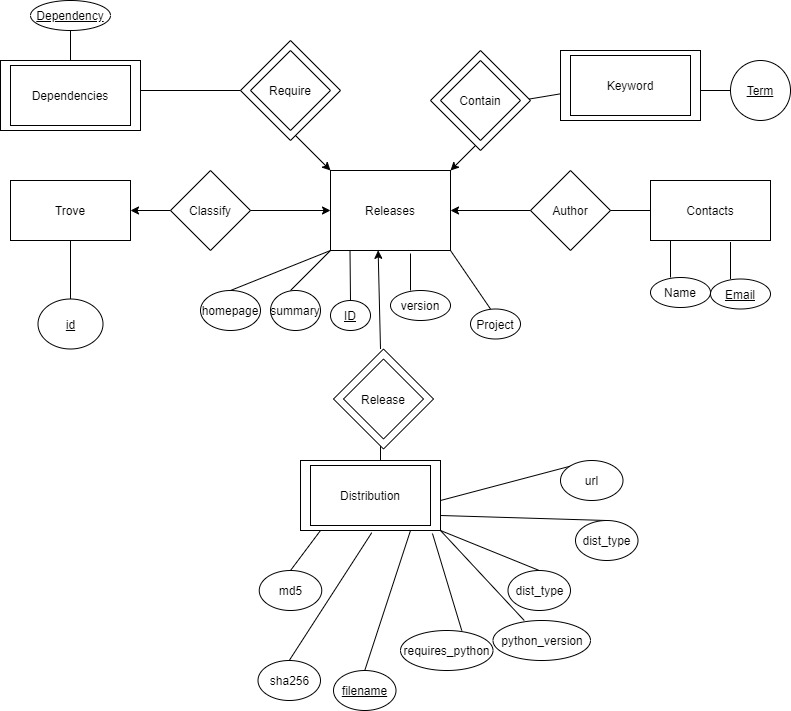
\includegraphics[width=0.9\textwidth]{ER Diagram.jpg}

This ER Diagram represents the relationship between each of its entity set of data extracted from projects:

Author(Releases-Contact:Many-One):Within each release,there could be one author,due to data extraction method doesn't support multi-author. Yet an author could have multiple releases under his name

Require(Releases-Dependencies:Many-Many):Every releases would require a number of dependencies,and many dependencies can be used by many releases.

Classify(Releases-Trove: Many-Many): This relationship indicates the relationship between Trove classifier and each releases,with many release could be classified
under one Trove classifier,and a release could be classified by many classifiers

Contain(Releases-Keyword:Many-Many): A release has many keywords,and also a keyword can also be in many releases.
  
Release(Releases-Distribution:One-Many): Within each releases, a number of distribution(s) would be released. A distribution could relate to only 1 releases,but many distributions could be released in the same releases

\subsection{Database Schema}

\subsubsection{releases}
This entity set represents each releases of the project,include the name of the project and its version in addition to summary,homepage and author's email. The ID of each releases is the primary key to represent each one of them.
This release ID is also the foreign key of many primary key in other entity set.
\subsubsection{keywords}
Containing both the ID of the releases and the terminology  as primary key,this entity represent the keywords of a specific release.
\subsubsection{contact}
Containing contact information of the author,including email (primary key) and name
\subsubsection{information}
Specific information of each releases. Containing release ID,summary,homepage and author's email of the releases.
\subsubsection{trove}
This entity set represent Trove classifiers,identified by its ID.
\subsubsection{classifiers}
Containing the release ID and Trove classifiers ID,this table has the role of representing the relationship of trove and releases
\subsubsection{Distribution}
This entity set represents the distribution of each releases. With its primary key its release ID along with its filename,each distribution contains the url,python version and the python version it requires,the distribtions it requires and its digests (a dictionary) sha256 and md5


\section{Data Query}

\section{Conclusion}

\begin{thebibliography}{69}
\end{thebibliography}
\end{document}
